A relevant characteristic of development processes is the time it takes to perform certain key tasks of the process. For example, in order to monitor whether a new version of a software will be successfully released within a given deadline, a project manager needs to know what is the progress with respect to the estimated delivery. All information that concerns the timing of work is referred to as the \emph{time perspective} the process. 

The class of processes that we discuss in this section are long-term engineering projects. These processes have specific requirements for monitoring. First, they are executed only once according to the specific needs of a particular project, and only partially according to recurring process descriptions. Second, they involve various actors that typically document their work in a semi-structured way using text and tables. Third, work in the project is usually subject to constraints regarding the start and end and the temporal order. Fourth, there is typically no process engine controlling the execution. Fifth, even though these limitations in terms of traceability exist, there are usually strong requirements in terms of tracking when which work was conducted.

%Unlike other types of business processes, the processes we consider here
%representing such projects are specifically tailored to customer needs the specific needs of the project, and there is

In line with these observations, a \textit{project-oriented business process} can be defined as an ad-hoc plan that specifies the tasks to be performed within a limited period of time and with a limited set of resources for achieving a specific goal. Unlike repetitive business processes for which notations such as \gls{bpmn}~\citep{bpmn2_stable} or \gls{epc}~\citep{vanderaalst_formalization_1999} are commonly used, project-oriented business processes may be properly represented with \gls{pert} or GANTT models. The concept is illustrated in Fig.~\ref{fig:bpm2015problem}.
%To manage the time perspective, complex software development projects are often planned by the use of a Gantt chart. 
The GANTT chart gives information about activities and work packages. Each work-package groups together similar types of activities. For example, all activities done in order to write the documentation of the project, will pertain to the work-package documentation. This inclusion also defines a hierarchy on the tasks. For example, the code of a feature \emph{A} may be located in a file \emph{F}. In turn, file \emph{F} may be in a folder \emph{D} which itself may be included on a super-folder \emph{Code}. This gives the hierarchy \emph{Code/D/F/A}. A typical way in which such hierarchy is organized in a file system is exactly through folder-in-folder and file-in-folder inclusions. 

\begin{figure}[htbp!]
	\centering
	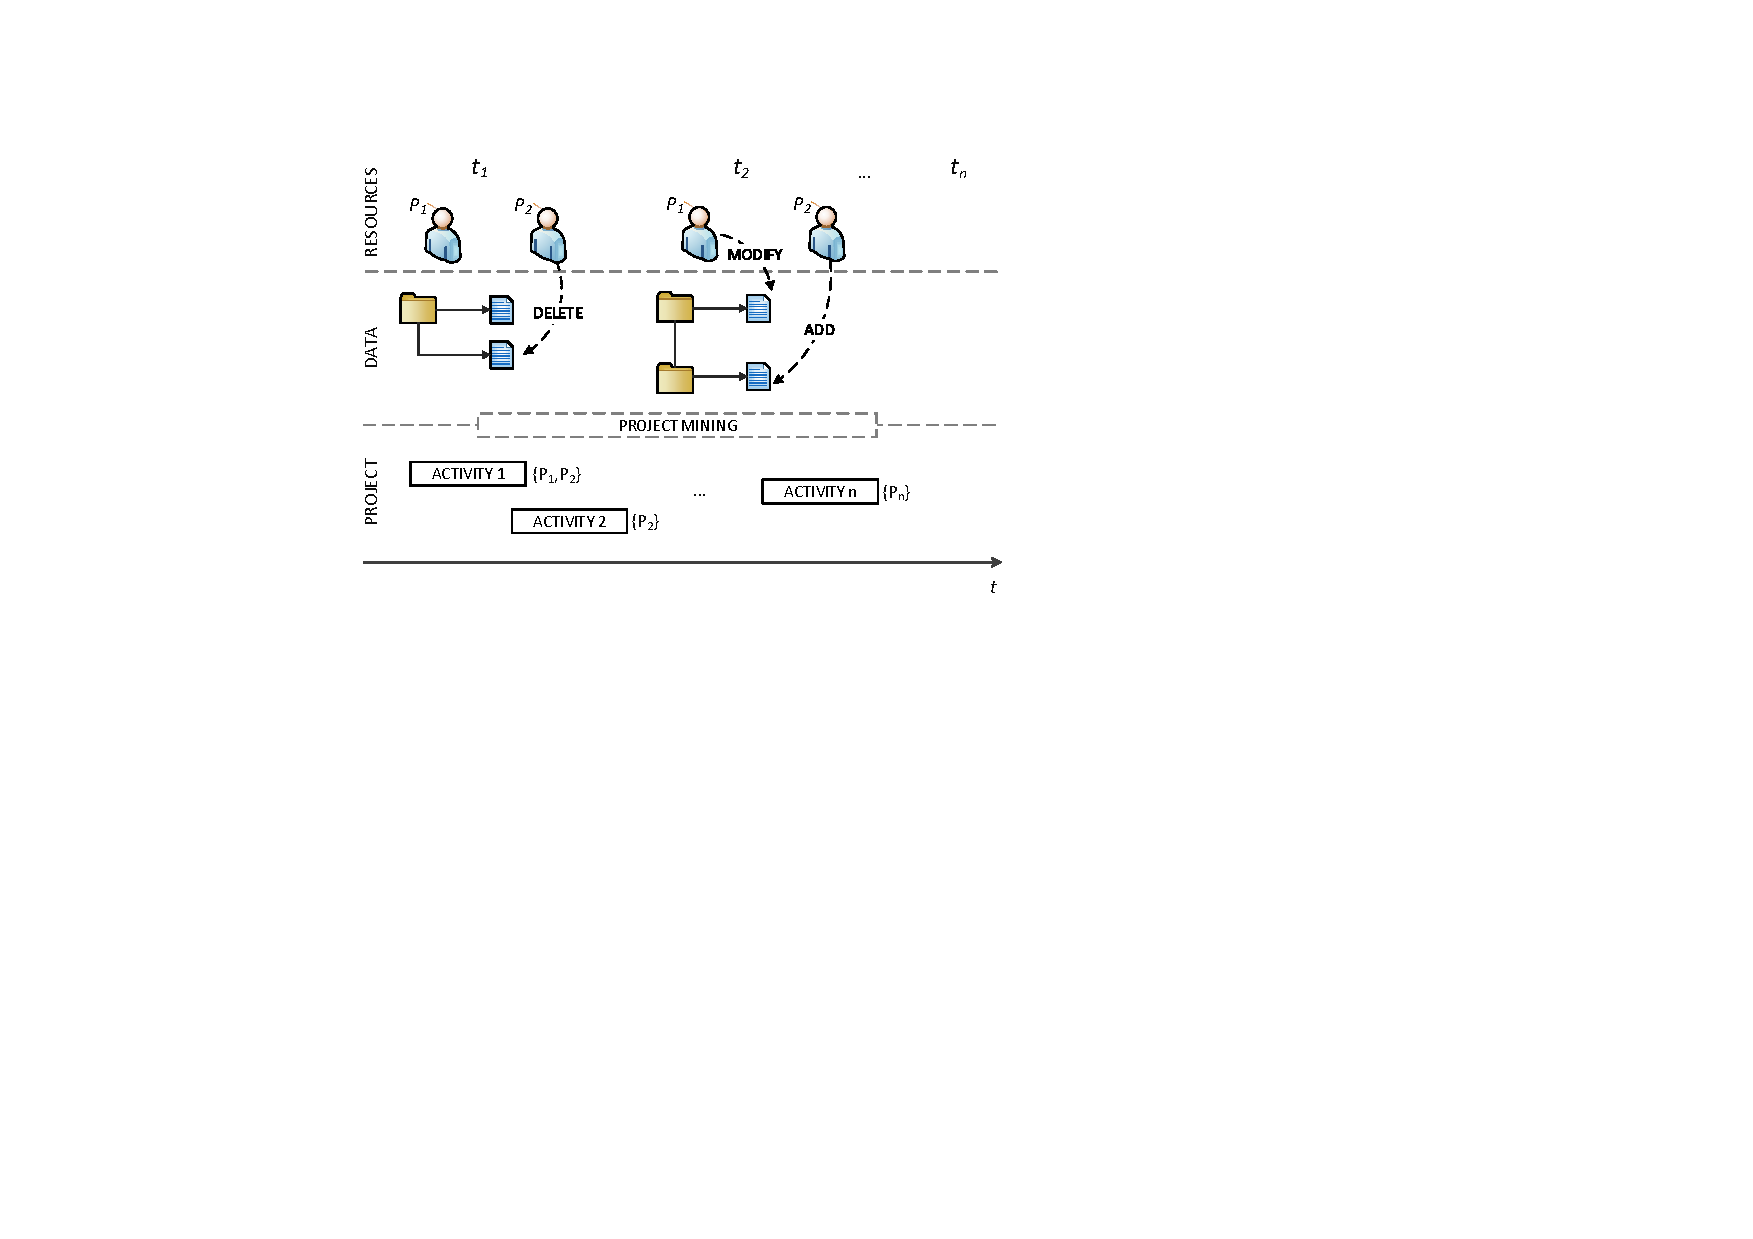
\includegraphics[width=.8\textwidth]{bpm2015/imgs/ProjectMining.pdf}
	\caption{Gap between User-Generated Artifacts and Project-Activities}
	\label{fig:bpm2015problem}
\end{figure}


%Software development processes can also be seen as project-oriented business processes. They share some common characteristics. First, they involve various resources with different roles. In the simplest case, we can distinguish \emph{project managers} and \emph{project participants}. Project managers are responsible for managing the development process and supervising the work of the project participants, who in turn are responsible for specific work tasks. Second, such processes are usually subject to constraints in terms of cost, time and quality, which is mostly associated with the performance of each of the work tasks. Third, the project participants work on a plethora of artifacts, which are logically organized in a hierarchical structure, with complex interdependencies among them.
Given these characteristics, it is the goal of the project manager to organize the software development process in such a way that the work on different files and tasks reflects the complex interdependencies, the constraints and the available participants. Therefore, it is important for the manager to understand the \emph{work history} of the process in order to monitor the progress systematically.
 


In order to perform the tasks of process monitoring, we need to gather meaningful time information from event logs. Resulting insights must be presented as a Gantt chart. This allows for comparing the actual Gantt chart of stemming from the data to planned one. Thus, possible deviations in terms of timing become easy to spot. Examples of deviations are related to the following questions: \emph{when did an activity start?} \emph{When did it finish?} \emph{How much work was performed in an time interval?} \emph{Are there any activities that are running late?} \emph{When did a bottleneck occur?} 
%- The minimum unit of work is a change to a file 


In line with the above description, we define the following requirements of a solution. 
\begin{itemize}
	\item[\textbf{Aggregate events.}] The developed artifact must be able to aggregate low-level file changes onto work-activities. 
	\item[\textbf{Organize activities into work-packages.}] The identified activities must be organized hierarchically organized within a work-package hierarchy. 
	\item[\textbf{Compute KPIs.}] The developed artifact must provide quantitative measures of the characteristics of a work-package.
\end{itemize}

\section{Related work} 
\label{sec:bpm2015related}

The problem described has been addressed in the literature from different perspectives. The first category of related work tackles the problem by transforming it into a process mining problem. Consequently, approaches have been developed to preprocess VCS data such that process mining techniques can be applied, and hence, a business process can be derived from the log data.
In this group, \cite{DBLP:conf/se/KindlerRS06,kindler2006incremental} developed an algorithm for extracting software processes that are mapped to Petri Nets. Activities, which are not explicit in the logs, are discovered from their input and output artifacts. However, strong assumptions are made on the filenames as well as on the software process lifecycle. %(always design, code, review, testres). Activities (which are not explicit in the logs, like in our case) are discovered from their input and output artifacts. Here defined as triples $<I,O,R>$ where I=input, O=Output, R=resouce who perfomed it.
\cite{rubin2007process} addressed the problem of engineering processes that are not well documented and are usually unstructured. They provided a bridge from Kindler et al.'s approach to ProM \citep{van2005prom} in order to mine different process perspectives, such as performance social network analyses. %but not from a project point of view.
\cite{rubin2014agile} applied process mining to the touristic industry and obtained user processes from web client logs pursuing the goal of improving the software system by analyzing the underlying process.
\cite{Poncin2011a} developed the FRASR framework for preprocessing software repositories to transform the VCS data to logs that conform to the process mining event log meta model~\citep{van2005meta} as utilized in ProM \citep{van2005prom}.
However, these approaches disregard the single-instance nature of project-oriented business processes and treat them as procedures that can be repeated over time.

The second category of related work focuses on the visualization of VCS data %by defining measurements such as things that can be plotted into a chart.
for different purposes.
%There are two main lines of how this problem was approached in literature.
%\paragraph*{visualization perspective} defining measurements such as things that can be plotted into a chart. But, they haven't any explicit notion of work structure.
%\paragraph*{preprocessing} - VCS data is transformed in order to comply to the process mining meta model from van Dongen and van der Aalst \citep{van2005meta}. This means that they are oriented to discover "classical" processing (i.e. repeated many times in the logs).
Several approaches study the interaction among developers over time from a visualization point of view. For instance,  \cite{ogawa2010software} drew storyline pathways to show the story of each developer's contribution. Other approaches analyze and visualize VCS data at file level in order to discover file version evolution. \cite{voinea_multiscale_2006} introduced an interactive navigation method to surf file version evolution as well as two methods to cluster versions of the same file in an abstraction layer. \cite{jingwei_evolution_2004} also visualized the evolutions of entire projects at file level, emphasizing the evolution moments.
Finally, several approaches study change prediction with the aim of discovering prediction patterns that can help in the process of software development~\citep{DBLP:journals/tse/ZimmermannWDZ05,ying_predicting_2004}.
%Feld et al. \citep{feldt2013supporting} used software project data to \emph{predict} potential problems during development. Heatmaps, used to visualize source code changes in a two dimensional space, showed to be easily readable also by non experts.
The approaches mentioned in this category as well as others that apply similar techniques~\citep{feldt2013supporting,kagdi_mining_2006,dambros_flexible_2008} focus on studying software evolution from different standpoints. However, the goal pursued differs in all cases from our goal in that they are not interested in discovering projects tasks out of the log data, and hence, they lack an explicit notion of work structure that we need to consider for our purpose.

Our approach combines ideas from both areas, as we aim at identifying tasks like in the approaches that rely on process mining, but we must cluster the data in an appropriate way, for which techniques developed in the approaches that pursue visualization may be adapted or extended.

%----------------
%
%Then explain that, in our work, we don't only want to see what's happening. We want also compliance (which means: did things happen in the right way (as they were allowed to)? Compliance can be provided by Process Mining algorithms... but we cannot apply process mining techniques directly (because they need logs structured in different ways - not svn/git logs). Thus, we need to adopt this strategy. 